\documentclass{article}
\usepackage{amsmath}
\usepackage{amsfonts}
\usepackage{amssymb}

\usepackage{enumitem}

\usepackage{graphicx}

\usepackage{minted}

\usepackage{hyperref}

\begin{document}

\tableofcontents

\newpage

\section{Probability}
\subsection{Probability}
\begin{enumerate}
	\item Fill in the details of the proof of Theorem 1.8. Also, prove the monotone decreasing case.
		\begin{itemize}
			\item For the readers' convenience we restate the Continuity of Probabilities theorem. If $A_n \rightarrow A$ then $P(A_n) \rightarrow P(A)$ as $n \rightarrow \infty$. Here $A_n \rightarrow A_n$ means that either $A_n$ is monotone increasing ($A_n \subseteq A_{n + 1}$) and we define $A = \bigcup_{n = 1}^\infty A_n$, or, $A_n$ is monotone decreasing ($A_n \supseteq A_{n + 1}$) and we define $A = \bigcap_{n = 1}^\infty A_n$.
			\item We fill in the details now. First of all we want to show that $B_i \cap B_j = \emptyset$ for all $i \neq j$. Suppose without loss of generality that $i < j$ and note that $B_i \subseteq A_i$ then
			$$
			B_j = A_j \backslash \bigcup_{k = 1}^{j - 1} A_k
			$$
			and $B_i \subseteq A_i \subseteq \bigcup_{k = 1}^{j - 1}$ as such $B_i \cap B_j = \emptyset$.
			\item To see that $A_n = \bigcup_{i = 1}^n B_i$ let $x \in A_n$ then there exists a minimal $k = k(x)$ such that $x \in A_k$, i.e., for all $k' < k : x \notin A_{k'}$. Then $x \notin \bigcup_{i = 1}^{k - 1} A_i$ and therefore $x \in B_k$. Because $x$ are arbitrary it folows that $A_n \subseteq \bigcup_{i = 1}^n B_i$. On the other hand
			$$
			\bigcup_{i = 1}^n \underbrace{B_i}_{\subseteq\ A_i} \subseteq \bigcup_{i = 1}^n A_i = A_n,
			$$
			where we have used that $A_n$ is monotone increasing. The property that
			$$
			\bigcup_{i = 1}^\infty A_i = \bigcup_{i = 1}^\infty B_i
			$$
			holds is identical to the finite case, an element is part of the (countably) infinite union if there exists some minimual $i$ such that ...
			\item For the monotone decreasing case we instead want to define $B_n := A_n \backslash \bigcup_{i > n} A_i$.
		\end{itemize}
	\item Prove the statements in equation (1.1).
		\begin{itemize}
			\item This can immediately be seen by noting that $A \cup B = (A \backslash B) \cup (A \cap B) \cup (B \backslash A)$ is a disjoint union.
		\end{itemize}
	\item Let $\Omega$ be a sample space and let $A_1, A_2, \dots, $ be events. Define $B_n = \bigcup_{i = n}^\infty A_i$ and $C_n = \bigcap_{i = n}^\infty A_i$
		\begin{enumerate}
			\item Show that $(B_i)$ is monotone decreasing and that $(C_i)$ is monotone increasing.
			\item Show that $\omega \in \bigcap_{n = 1}^\infty B_n$ if and only if $\omega$ belongs to an infinite number of events $A_1, A_2, \dots$.
				\begin{itemize}
					\item Let $\omega \in \bigcap_{n = 1}^\infty B_n$ be such that $\omega$ does not belong to an infinite number of events $A_1, A_2, \dots$, i.e., there exists $N \in \mathbb{N}$ such that for all $k > N$ it follows that $\omega \notin A_k$. But then $\omega \notin B_k$ for all $k > N$ and as such does not lie in the intersection over all the $B_k$, which is a contradiction.
					\item Suppose $\omega$ lies in infinitely many $A_1, A_2, ...$. Then there exists a sequence $(A_{n_i})_{i \in \mathbb{N}}$ such that $n_i < n_{j}$ for all $i < j$ and such that $\omega \in A_{n_i}$ for all $i \in \mathbb{N}$. In that case
					$$
					\omega \in B_{n_i}
					$$
					for all $i \in \mathbb{N}$, in particular $\omega \in \cap_{i = \mathbb{N}} B_{n_i}$. Because $B_n$ is monotone decreasing the statement follows.
				\end{itemize}
			\item Show that $\omega \in \bigcup_{n = 1}^\infty C_n$ if and only if $\omega$ belongs to all the events $A_1, A_2, \dots$ except possibly a finite number of those events.
				\begin{itemize}
					\item Let $\omega \in \bigcup_{n = 1}^\infty B_n$ then there exists $n \geq 1$ such that $\omega \in B_n$. This means that $\omega \in \bigcap_{i = n}^\infty$, i.e., $\omega$ belongs to all $A_i$ where $i \geq n$.
					\item Now suppose $\omega$ belongs to all events $A_1, A_2, \dots$ except for a finite number of events. In that case there exist $N \in \mathbb{N}$ such that $\forall k \geq N : \omega \in A_k$. This means that
					$$
					\omega \in \bigcap_{i \geq k} A_i,
					$$
					i.e., $\omega \in C_k$. In particular this shows
					$$
					\omega \in C_k \subseteq \bigcup_{r \geq 1} C_r.
					$$
				\end{itemize}
		\end{enumerate}
	\item Let $\{A_i : i \in I\}$ be a collection of events where $I$ is an arbitrary index set. Show that
	$$
	\begin{aligned}
	\left( \bigcup_{i \in I} \right)^c = \bigcap_{i \in I} A_i^c, && \left( \bigcap_{i \in I} A_i \right)^c = \bigcup_{i \in I} A_i^c
	\end{aligned}
	$$
	holds.

	Hint: First prove this for $I = \{1, 2, \dots, n\}$.
	\item Suppose we toss a fair coin until we get exactly two heads. Describe the sample space S. What is the probability that exactly k tosses are required?
	\item Let $\Omega = \{0, 1, \dots \}$. Prove that there does not exist a uniform distribution on $\Omega$ (i.e., if $P(A) = P(B)$ whenever $|A| = |B|$, then $P$ cannot satisfy the axioms of probability.)
		\begin{itemize}
			\item Note that $P(\{0\}) \neq 0$ because otherwise $P = 0$, which would mean $P$ is not a probability function. But then it follows for all $n \in \mathbb{N}$:
			$$
			P(\{0, \dots, n\}) = P\left(\bigcup_{k = 0}^n \{k\} \right) = \sum_{k = 0}^n P(\{k\}) = (n + 1)P(\{0\}) \rightarrow \infty
			$$
			for $n \rightarrow \infty$, which is a contradiction to $P(\Omega) = +1$.
		\end{itemize}
	\item Let $A_1, A_2, \dots$ be events. Show that
	$$
	\left( \bigcup_{n = 1}^\infty A_n \right) \leq \sum_{n = 1}^\infty P(A_n).
	$$
	Hint: Define $B_n = A_n \backslash \bigcup_{i = 1}^{n - 1} A_i$. Then show that the $B_n$ are disjoint and that
	$$
	\bigcup_{n = 1}^\infty A_n = \bigcup_{n = 1}^\infty B_n.
	$$
	\begin{itemize}
		\item This was basically already shown in the first exercise, the only thing we mention here is that we only have to consider the case where the series on the right hand side converges, because the left hand side is always $\leq 1$.
	\end{itemize}
	\item Suppose that $P(A_i) = 1$ for each $i$. Prove that
	$$
	P\left( \bigcap_{i = 1}^\infty A_i \right) = 1.
	$$
	\item For fixed $B$ such that $P(B) > 0$, show that $P(\cdot|B)$ satisfies the axioms of probability.
	\item You have probably heard it before. Now you can solve it rigorously. It is called the "Monty Hall Problem." A prize is placed at random behind one of three doors. You pick a door. To be concrete, let's suppose you always pick door $1$. Now Monty Hall chooses one of the other two doors, opens it and shows you that it is empty. He then gives you the opportunity to keep your door or switch to the other unopened door.Should you stay or switch? Intuition suggests it doesn't matter. The correct answer is that you should switch. Prove it. It will help to specify he sample space and the relevant events carefully. Thus write $\Omega = \{(Wl,W2): \omega_i \in \{1,2,3\}\}$ where $\omega_1$ is where the prize is and $\omega_2$ is the door Monty opens.
	\item Suppose that $A$ and $B$ are independentt events. Show that $A^c$ and $B^c$ are independent events.
		\begin{itemize}
			\item
			$$
			\begin{aligned}
			P(A^c, B^c) &= P((A \cup B)^c) \\
			&= 1 - P(A \cup B) \\
			&= 1 - P(A) - P(B) + P(A, B) \\
			&= 1 - P(A) - P(B) + P(A)P(B) \\
			&= (1 - P(A))(1 - P(B)) \\
			&= P(A^c)P(B^C).
			\end{aligned}
			$$
		\end{itemize}
	\item There are three cards. The first is green on both sides, the second is red on both sides and the third is green on one side and red on the other. We choose a card at random and we see one side (also chosen at random) . If the side we see is green, what is the probability that the other side is also green? Many people intuitively answer $\frac{1}{2}$. Show that the correct answer is $\frac{2}{3}$.
	\item Suppose that a fair coin is tossed repeatedly until both a head and tail have appeared at least once.
		\begin{enumerate}
			\item Describe the sample space $\Omega$.
			\item What is the probability that three tosses will be required?
		\end{enumerate}
	\item Show that if $P(A) = 0$ or $p(A) = 1$ then $A$ is independent of every other event. Show that if A is independent of itself then $P(A)$ is either $0$ or $1$.
		\begin{itemize}
			\item 
			\item $P(A) = P(A, A) = P(A)P(A) = P(A)^2 \iff P(A)(P(A) - 1).$
		\end{itemize}
	\item
	\item Prove Lemma 1.14.
		\begin{itemize}
			\item
			$$
			P(A|B) = \frac{P(A, B)}{P(B)} = \frac{P(A)P(B))}{P(B)} = P(A).
			$$
			\item
			$$
			\begin{aligned}
			P(AB) &= P(A, B) \frac{P(B)}{P(B)} \\
			&= P(A|B) P(B) \\
			& = P(B|A) \frac{P(A)}{P(B)} P(B) \\
			&= P(B|A)P(A).
			\end{aligned}
			$$
		\end{itemize}
	\item Show that
	$$
	P(A, B, C) = P(A|BC)P(B|C)P(C).
	$$
	\item
	\item 
	\item 
	\item (Computer Experiment.) Suppose a coin has probability $p$ of falling heads up. If we flip the coin many times, we would expect the proportion of heads to be near $p$. We will make this formal later. Take $p = 0.3$ and $n = 1000$ and simulate $n$ coin flips. Plot the proportion of heads as a function of n. Repeat for $p = 0.03$.
		\begin{itemize}
			\item
\begin{minted}{python}
import numpy as np
import matplotlib.pyplot as plt
import math

def Ex1_21(p = 0.3, n = 1000, draw = True, save = False):
    rand = np.random.random(size = 1000)
    _range = np.arange(1, n + 1)

    result = np.cumsum(rand < p) / _range

    fig, ax = plt.subplots()

    ax.plot(_range, result)

    if draw:
        plt.show()

    if save:
        # p = 0.213, n = 1000 -> 21pct_1000
        str_form = f"{math.floor(p * 100)}pct_{n}"
        fig.savefig(f"Ex1_21-{str_form}.png")

Ex1_21(p = 0.3, draw = True, save = True)
Ex1_21(p = 0.03, draw = True, save = True)
\end{minted}
		\begin{tabular}{cc}
			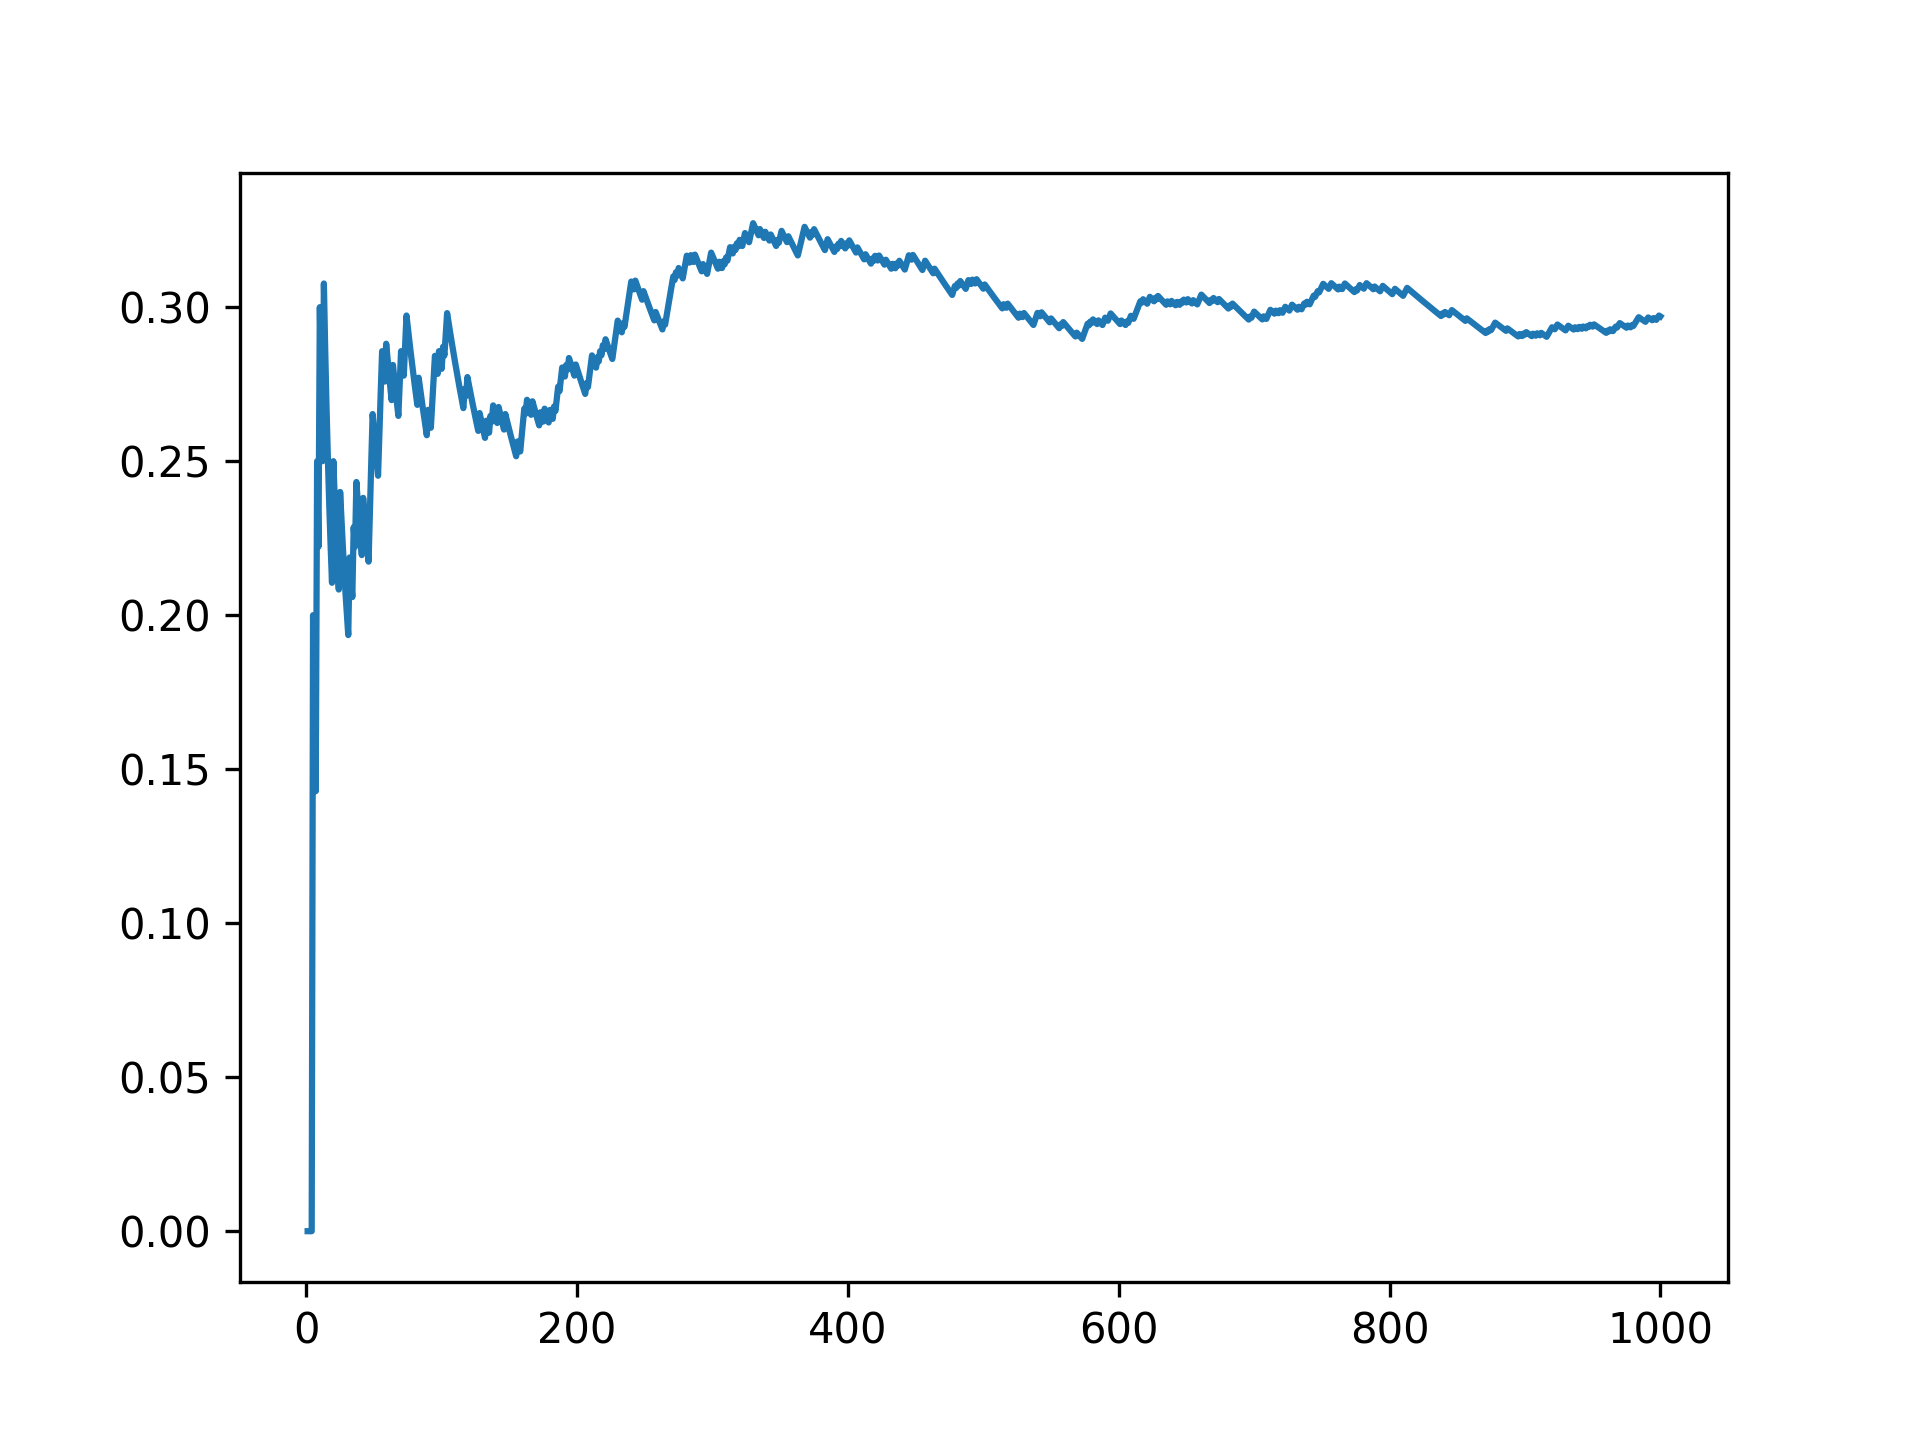
\includegraphics[width=0.45\textwidth]{1-Probability/Ex1_21-30pct_1000.png} &
			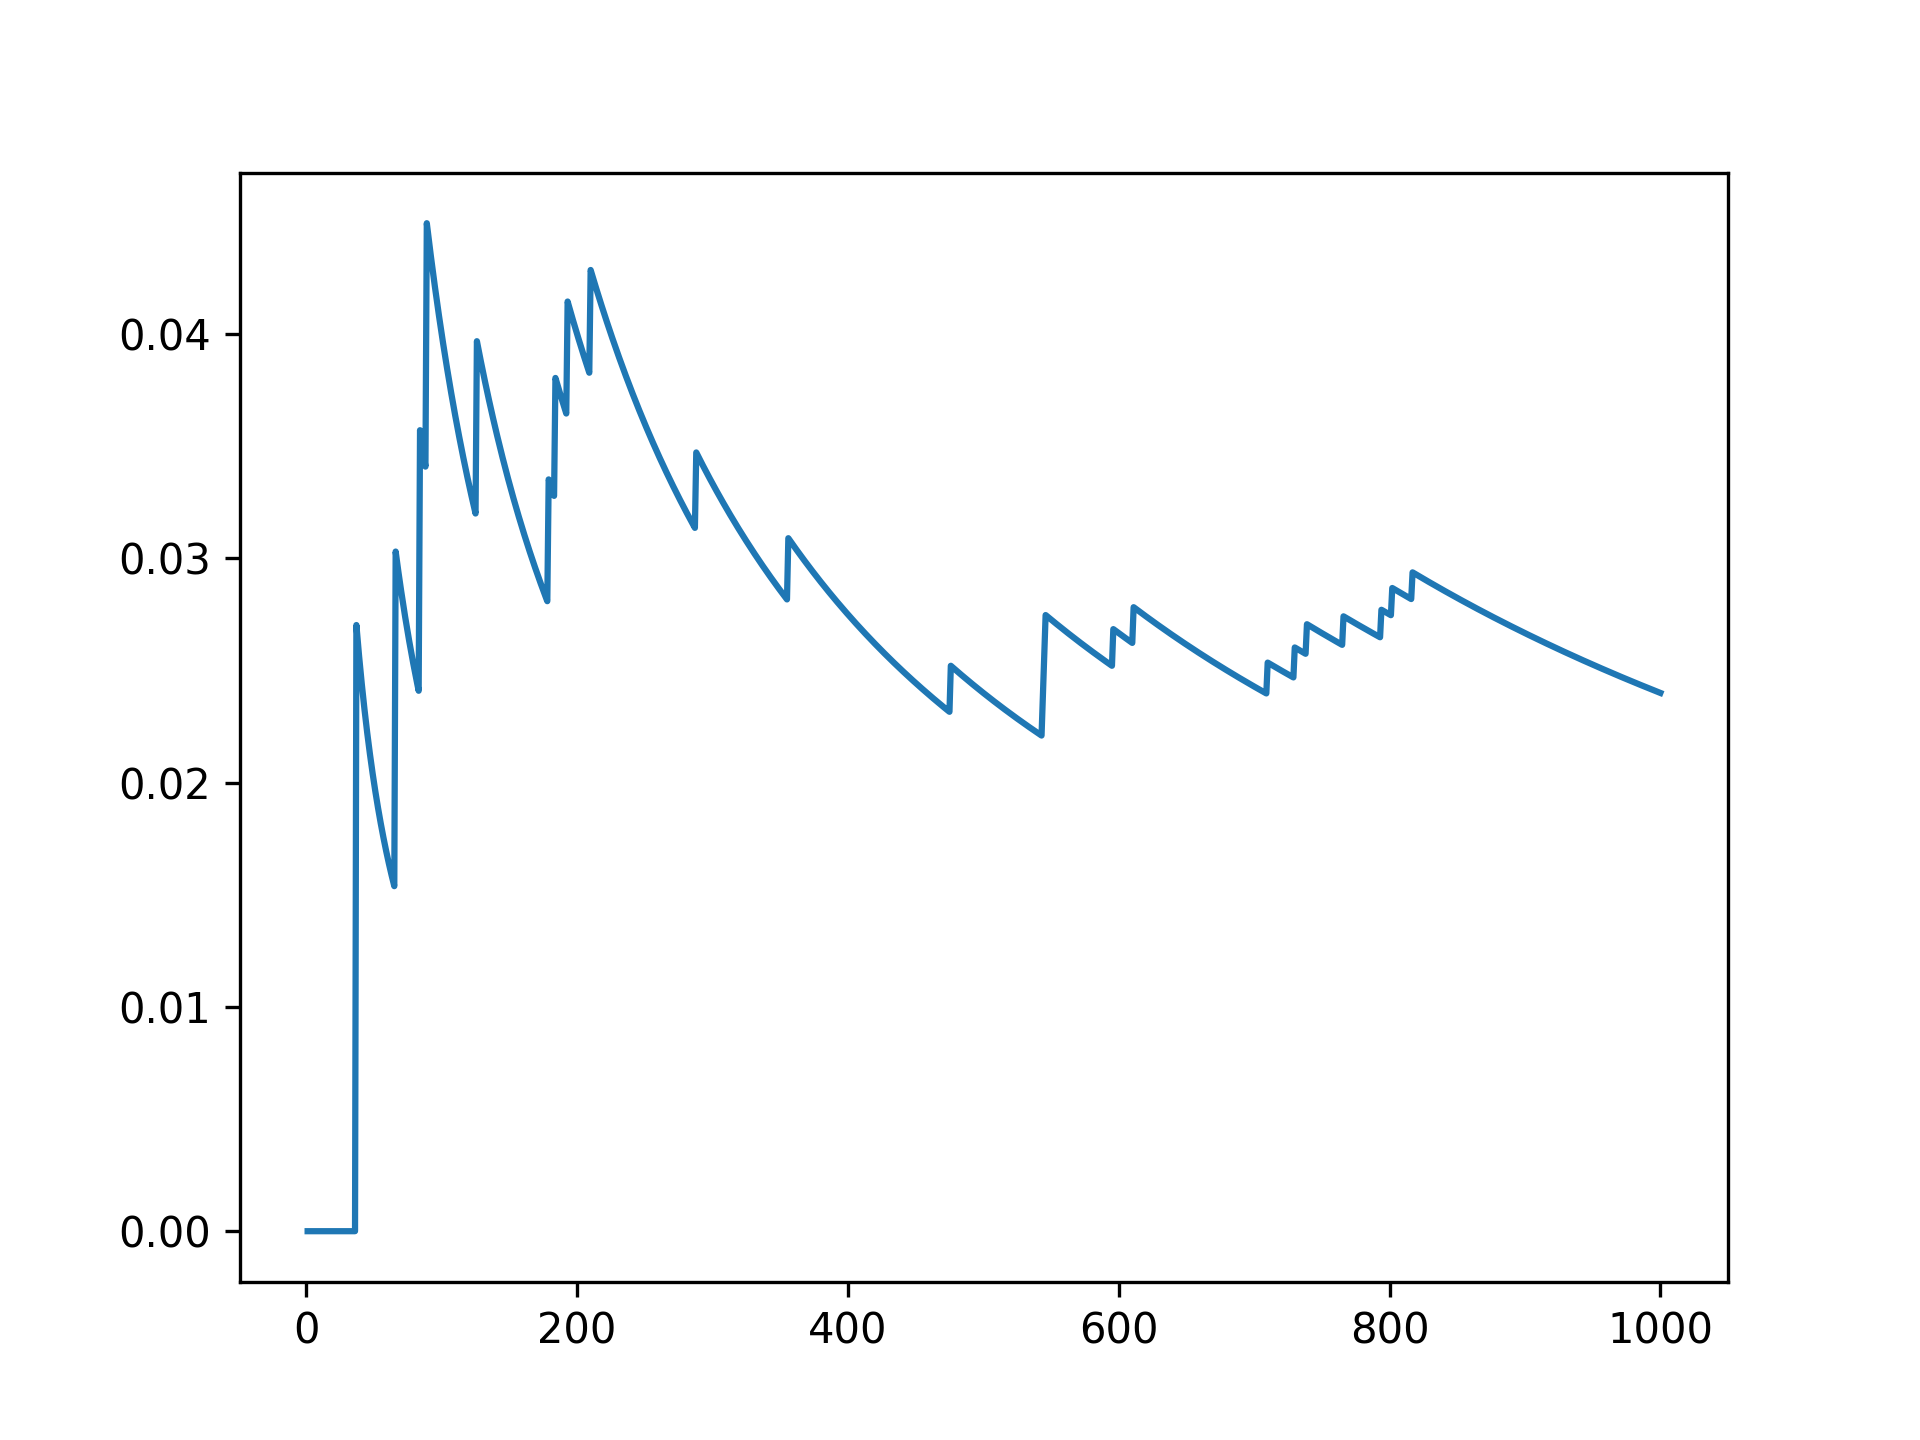
\includegraphics[width=0.45\textwidth]{1-Probability/Ex1_21-3pct_1000.png} \\
			(a) 30\% Probability & (b) 3\% Probability \\
		\end{tabular}
		\end{itemize}
	\item (Computer Experiment.) Suppose we flip a coin n times and let P denote the probability of heads. Let X be the number of heads. We call X a binomial random variable, which is discussed in the next chapter. Intuition suggests that X will be close to n p. To see if this is true, we can repeat this experiment many times and average the X values. Carry out a simulation and compare the average of the X's to n p . Try this for $p = 0.3$ and $n = 10$, $n = 100$, and $n = 1000$.
		\begin{itemize}
			\item 
\begin{minted}{python}
import numpy as np

def Ex1_22(p = 0.3, n = 1000, num_iter = 100):
    sum = 0
    for i in range(num_iter):
        rand = np.random.random(size = n)
        sum += np.sum(rand < p)

    mean = sum / num_iter
    expected = n * p
    delta = abs(mean - expected) / (expected)
    print(f"mean = {mean}, delta = {delta * 100:.2f}%")

for n in [10, 100, 1000]:
    Ex1_22(n = n)

> mean = 2.93, delta = 2.33%
> mean = 30.2, delta = 0.67%
> mean = 297.83, delta = 0.72%
\end{minted}
		\end{itemize}
	\item (Computer Experiment.) Here we will get some experience simulating conditional probabilities. Consider tossing a fair die. Let $A = \{2, 4, 6\}$ and $B = \{1, 2, 3, 4\}$. Then, $P(A) = 1/2$, $P(B) = 2/3$ and $P(AB) = 1/3$. Since $P(AB) = P(A)P(B)$, the events $A$ and $B$ are independent. Simulate draws from the sample space and verify that $\hat{P}(AB) = \hat{P}(A)\hat{P}(B)$ where $\hat{P}(A)$ is the proportion of times $A$ occurred in the simulation and similarly for $\hat{P}(AB)$ and $\hat{P}(B)$. Now find two events $A$ and $B$ that are not independent. Compute $\hat{P}(A)$,$\hat{P}(B)$ and $\hat{P}(AB)$. Compare the calculated values to their theoretical values. Report your results and interpret.
	\begin{itemize}
		\item
\begin{minted}{python}
import numpy as np

labels = ['P(A)', 'P(B)', 'P(A, B)', 'P(A)P(B)', 
          'P(A, B) - P(A)P(B)']
pct_str = lambda x : f"{x * 100:.2f}%"

def Ex1_23_helper(probabilities):
    for label, prob in zip(labels, probabilities):
        print(f"\t{label}: {pct_str(prob)}")

def Ex1_23(A, B, n = 10000):
    cap = A.intersection(B)

    # rand does [) so I need to increment high to get 6
    rand = np.random.randint(low = 1, high = 6 + 1, size = n)
    prob_A = sum(np.isin(rand, list(A))) / n
    prob_B = sum(np.isin(rand, list(B))) / n
    prob_cap = sum(np.isin(rand, list(cap))) / n

    prob_prod = prob_A * prob_B

    probabilities = [prob_A, prob_B, prob_cap, prob_prod,
                     prob_cap - prob_prod]

    print("Experimental Values")
    Ex1_23_helper(probabilities)

A, B = {2, 4, 6}, {1, 2, 3, 4}
print(f"A = {A}, B = {B}, AB = {A.intersection(B)}")
print("Theoretical Values")
Ex1_23_helper([1/2, 2/3, 1/3, 1/3, 0])
Ex1_23(A, B)
print()

A, B = {1, 2, 3}, {3, 4, 5, 6}
print(f"A = {A}, B = {B}, AB = {A.intersection(B)}")
print("Theoretical Values")
Ex1_23_helper([1/2, 2/3, 1/6, 1/3, -1/6])
Ex1_23(A, B)

> A = {2, 4, 6}, B = {1, 2, 3, 4}, AB = {2, 4}
> Theoretical Values
> 	P(A): 50.00%
> 	P(B): 66.67%
> 	P(A, B): 33.33%
> 	P(A)P(B): 33.33%
> 	P(A, B) - P(A)P(B): 0.00%
> Experimental Values
> 	P(A): 50.18%
> 	P(B): 67.42%
> 	P(A, B): 33.70%
> 	P(A)P(B): 33.83%
> 	P(A, B) - P(A)P(B): -0.13%
> 
> A = {1, 2, 3}, B = {3, 4, 5, 6}, AB = {3}
> Theoretical Values
> 	P(A): 50.00%
> 	P(B): 66.67%
> 	P(A, B): 16.67%
> 	P(A)P(B): 33.33%
> 	P(A, B) - P(A)P(B): -16.67%
> Experimental Values
> 	P(A): 50.20%
> 	P(B): 66.30%
> 	P(A, B): 16.50%
> 	P(A)P(B): 33.28%
> 	P(A, B) - P(A)P(B): -16.78%
\end{minted}
		\end{itemize}
\end{enumerate}

\section{Random Variables}
\begin{enumerate}
	\item Show that
	$$
	P(X = x) = F(x^+) - F(x^-).
	$$
	\item Let $X$ be such that $P(X = 2) = P(X = 3) = 1 / 10$ and $P(X = 5) = 8 / 10$. Plot the CDF $F$. Use $F$ to find $P(2 \leq X \leq 4.8)$ and $P(2 \leq X \leq 4.8)$.
	\item Prove Lemma 2.15.
	\item 
	\item Let $X$ and $Y$ be discrete random variables. Show that $X$ and $Y$ are independent if and only if $f_{X, Y}(x, y) = f_X(x)f_Y(y)$ for all $x$ and $y$.
\end{enumerate}

\end{document}